\documentclass{article}
\usepackage[utf8]{inputenc}
\usepackage[czech]{babel}
\usepackage{natbib}
\usepackage{graphicx}
\usepackage{listings}
\usepackage{xcolor}
\lstset {
    language=bash,
    backgroundcolor=\color{black!5}, % set backgroundcolor
    basicstyle=\footnotesize,% basic font setting
}

\title{IVS - profiling}
\author{Lidé u výtahu}
\date{April 2020}

\begin{document}

\maketitle

\tableofcontents

\section{Úvod}
Pro výpočet výběrové směrodatné odchylky naše skupina zvolila vývoj konzolové aplikace s názvem SampleStandardDeviation.exe. Tato aplikace používá třídu IVSMath s matematickými operacemi. Ze stdin načte libovolný počet čísel a na stdout vypíše výběrovou směrodatnou odchylku. Nepovinný argument N určí, kolikrát se má každá funkce třídy IVSMath spustit.

Příklady spuštění:

\begin{lstlisting}[language=bash]
  $ ./SampleStandardDeviation.exe < /data/data10.txt
  $ ./SampleStandardDeviation.exe 1000 < /data/data10.txt
\end{lstlisting}

\section{Profiling}
Ve Visual Studiu 2019 jsme naši aplikaci profilovali pomocí Performance profileru, který jako výstup vytváří soubor s příponou .diagsession. Tento soubor obsahuje veškerá data zjištěná při profilingu a dá se otevřít přímo ve Visual Studiu, ale z důvodu velikosti jsme je neuložili. Pro rychlejší a pohodlnější zobrazení jsme vytvořili screenshoty funkce Main s využitím jednotlivých řádků.

Soubory *.diagsession mimo jiné obsahují tabulku funkcí s jednotkami CPU, které daná funkce spotřebovala za běhu aplikace. Zobrazuje funkce, které spotřebují alespoň jednu jednotku CPU, ostatní nezahrnuje. To stejné platí pro zobrazení náročnosti jednotlivých řádků. 

\subsection{Jednoduchý profiling}
V první fázi jsme profilovali aplikaci bez argumentu N. Každá funkce se tedy vykonala pouze jednou. Výsledky jsou v souborech vystup-*.png. Viz Obrázek 1, kde je výsledek profilingu aplikace se vstupem ze souboru data/data1000.txt.

\begin{figure}[h]
\centering
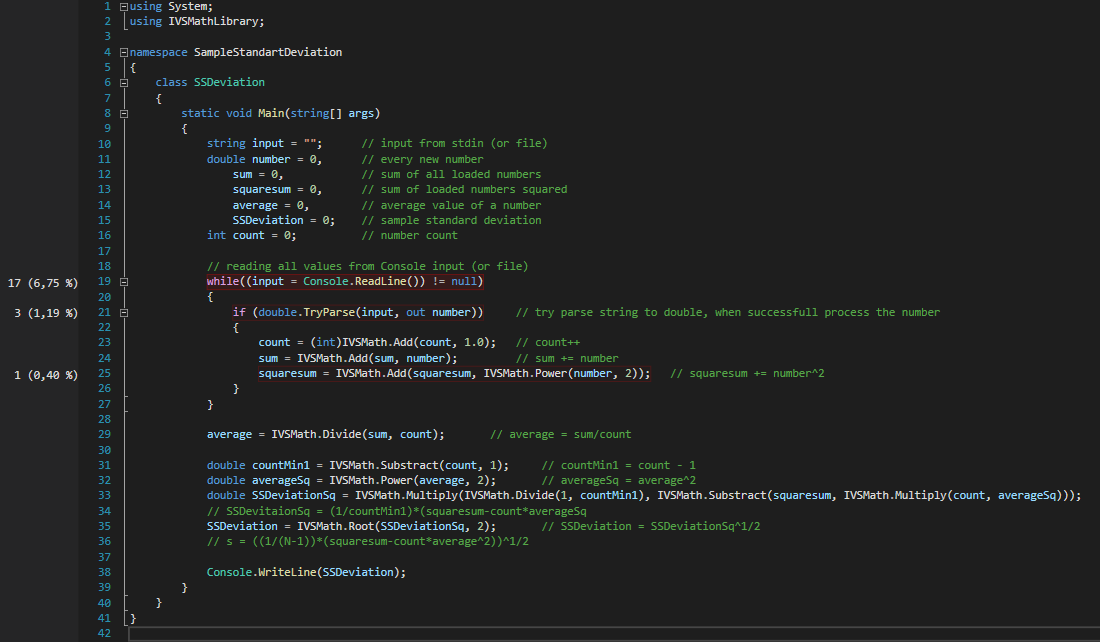
\includegraphics[scale=0.49]{vystup-data1000}
\caption{Výstup jednoduchého profileru}
\label{profiler:data1000}
\end{figure}

\subsection{Profiling s opakováním}
Jednoduchý profiling nám přinesl zajímavá ale veskrze ne moc použitelná data pro případnou optimalizaci. Proto jsme profilovali s argumentem N = 100, 1000 a 10000. Každá funkce se při každém volání zopakuje Nkrát. Výstup profileru s opakováním nám ukáže mnohem přesněji, kde je potřeba optimalizovat. 

Viz Obrázek 2, kde je výsledek profilingu aplikace se vstupem ze souboru data/data1000.txt a argumentem N=10000. Na tomto výstupu je vidět, že nejvíce času strávil program ve funkcích IVSMath.Add a IVSMath.Power. Na tyto funkce bychom se tedy měli soustředit při případné optimalizaci.

\begin{figure}[h]
\centering
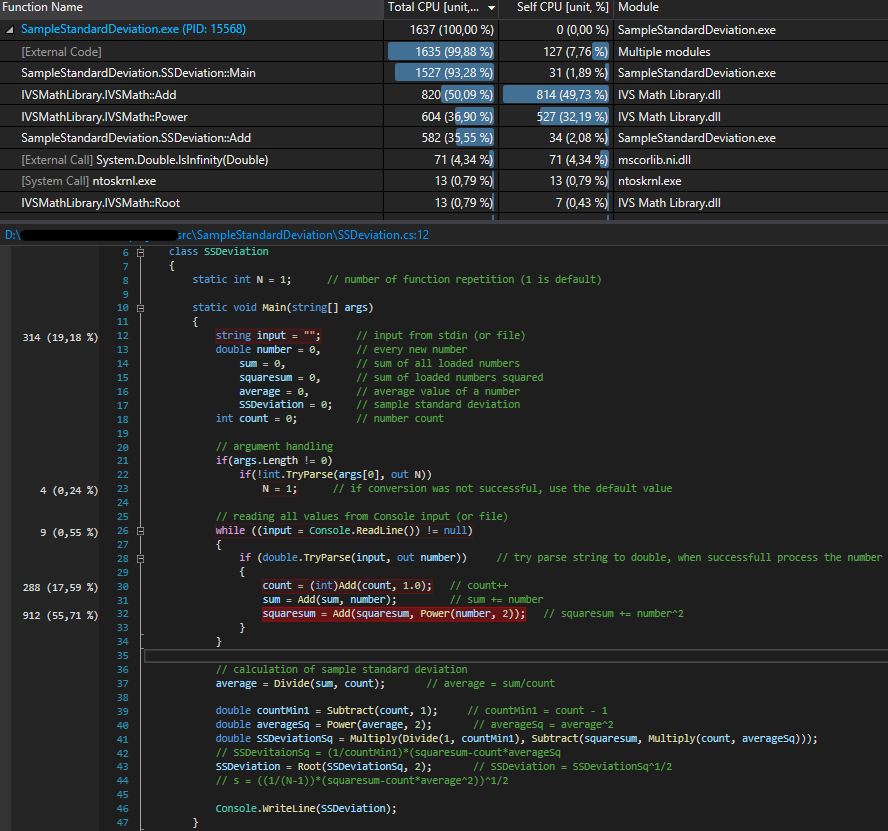
\includegraphics[scale=0.54]{vystup-data1000-withN-10000}
\caption{Výstup profileru s opakováním}
\label{profiler:data1000-withN-10000}
\end{figure}

\section{Závěr}
Obě metody profilingu jsou v praxi přínosné. V našem případě bylo k dosažení cíle potřeba rozšířit původní zadání. Pomocí metody profilingu s opakováním jsme zjistili, které funkce jsou nejvíce náročné a měli by se optimalizovat pro zvýšení výkonu aplikace.

\section{Přílohy}
\begin{tabular}[pos]{ | c | c |}
\hline
{\bf Název souboru} & {\bf Popis} \\
\hline
vystup-data10.png & screenshot profilingu s 10 vstupy \\
\hline
vystup-data100.png & screenshot profilingu se 100 vstupy \\
\hline
vystup-data1000.png & screenshot profilingu s 1000 vstupů \\
\hline
vystup-data1000-withN-100.png & screenshot s opakováním 100x \\
\hline
vystup-data1000-withN-1000.png & screenshot s opakováním 1000x \\
\hline
vystup-data1000-withN-10000.png & screenshot s opakováním 10000x \\
\hline
\end{tabular}
\end{document}
